\documentclass[12pt,letterpaper]{article}
\usepackage[framemethod=tikz]{mdframed}
\usepackage[utf8]{inputenc} %Spanish input
\usepackage[T1]{fontenc} % Use 8-bit encoding that has 256 glyphs
\usepackage[spanish, es-tabla]{babel} % Selecciona el español para palabras introducidas automáticamente, p.ej. "septiembre" en la fecha y especifica que se use la palabra Tabla en vez de Cuadro
\usepackage{fullpage}
\usepackage[top=2cm, bottom=4.5cm, left=2.5cm, right=2.5cm]{geometry}
\usepackage{lastpage}
\usepackage{enumerate}
\usepackage[inline]{enumitem}
\usepackage{fancyhdr}
\usepackage{xcolor}
%
\usepackage[sorting=none]{biblatex}
\addbibresource{citas.bib}
%
\usepackage{csquotes}
\usepackage{cellspace}
\setlength{\cellspacetoplimit}{5pt}
\setlength{\cellspacebottomlimit}{5pt}
\usepackage{hhline}
\usepackage{listings}
\usepackage{hyperref}
\usepackage{titletoc,tocloft}
\usepackage{float,subfig}
\setlength{\cftsubsecindent}{2cm}
\setlength{\cftsubsubsecindent}{4cm}
\dottedcontents{section}[1.5em]{}{1.3em}{.6em}
%\usepackage[nodisplayskipstretch]{setspace}
%
\graphicspath{ {./imgs/} } %Drawing the background pic
\usepackage{tikz}
\newcommand{\tikzmark}[1]{\tikz[baseline,remember picture] \coordinate (#1) {};}
\usetikzlibrary{positioning}
\usetikzlibrary{shadows,arrows.meta} % For adding edges label
\usetikzlibrary{calc}
\usepackage{eso-pic}
\AddToShipoutPictureBG{%
    \begin{tikzpicture}[remember picture, overlay]
        \node[opacity=.15, inner sep=0pt]
            at(current page.center){
\includegraphics[scale=1.5]{logo-ugr2}};
    \end{tikzpicture}%
}

% \numberwithin{equation}{section} % Number equations within sections (i.e. 1.1, 1.2, 2.1, 2.2 instead of 1, 2, 3, 4)
% \numberwithin{figure}{section} % Number figures within sections (i.e. 1.1, 1.2, 2.1, 2.2 instead of 1, 2, 3, 4)
% \numberwithin{table}{section} % Number tables within sections (i.e. 1.1, 1.2, 2.1, 2.2 instead of 1, 2, 3, 4)

\hypersetup{%
    colorlinks=true,
    linkcolor=[rgb]{0.2, 0.3, 0.5},
    urlcolor=black,
    citecolor=black,
    linkbordercolor={0 0 1}
}

\renewcommand\lstlistingname{Código:}
\renewcommand\lstlistlistingname{Código:}
\def\lstlistingautorefname{Brian SS.}
%
%
\newcommand{\horrule}[1]{\rule{\linewidth}{#1}} % Create horizontal rule command with 1 argument of height
\definecolor{codegreen}{rgb}{0,0.6,0}
\definecolor{codegray}{rgb}{0.5,0.5,0.5}
\definecolor{codepurple}{rgb}{0.58,0,0.82}
\definecolor{backcolour}{rgb}{0.95,0.95,0.92}
%
\lstset{language=python,basicstyle=\linespread{1.1}\ttfamily\footnotesize,
    xleftmargin=0.0cm, frame=t, framesep=0.15cm, framerule=0pt, tabsize=4,
    showspaces=false, showstringspaces=false,showlines=true,
    keywordstyle=\color{blue}\ttfamily,
    stringstyle=\color{red}\ttfamily,
    commentstyle=\color{gray}\ttfamily,
    morecomment=[l][\color{magenta}]{\#}
}
%
\setlength{\parindent}{0.0in}
\setlength{\parskip}{0.05in}
%
%% Edit these as appropriate
\newcommand\course{Ciencia de Datos e Ingenieria de Computadores}
\newcommand\hwnumber{1}                  % <-- homework number
\newcommand\NetIDa{}           % <-- NetID of person #1
\newcommand\NetIDb{}           % <-- NetID of person #1
%
\pagestyle{fancyplain}
\headheight 35pt
\lhead{\NetIDa}
%\lhead{\NetIDa\\\NetIDb}                 % <-- Comment this line out for problem sets (make sure you are person #1)
\lhead{\textbf{\large Preprocesamiento y Clasificación}}
\rhead{\course \\ \today}
\lfoot{\scriptsize\LaTeX}
\cfoot{\hyperlink{Indice}{Volver al índice}}
\rfoot{\small\thepage}
\headsep 1.5em
%
\renewcommand*\contentsname{Índice}
%
\author{Brian Sena Simons} % Nombre y apellidos
%
\date{\normalsize\today} % Incluye la fecha actual
%
\begin{document}
%
\begin{titlepage}
\begin{figure}[H]
    \vspace{-1.3cm}
    \begin{center}
        
\includegraphics[width=0.75\textwidth]{Etsiit}
    \end{center}
\end{figure}
\vspace{1.3cm}
\centering
\normalfont \normalsize
\textsc{\textbf{Minería de Datos} \\ \vspace{.15cm} Master en Ciencia de Datos e Ingeniería de Computadores \\ \vspace{.15cm} Universidad de Granada} \\ [25pt] % Your university, school and/or department name(s)
    \horrule{0.5pt} \\[0.4cm] % Thin top horizontal rule
    \huge Preprocesamiento y Clasificación\\ % The assignment title
    \horrule{2pt} \\[0.5cm] % Thick bottom horizontal rule

\begin{minipage}{0.4\textwidth}
    \begin{flushleft}\large
        \emph{Autores:} \\
         ----------------------- \\
        \vspace{.15cm}
        Brian Sena Simons. \\
        Miguel Garcia Lopez. \\
        Álvaro Santana Sánchez. \\ 
        Ana Fuentes Rodríguez.

    \end{flushleft}
\end{minipage}
\begin{minipage}{0.4\textwidth}
    \vspace{-2.2cm}
     \begin{flushright}\large
         Grupo: \\
         ----------------------- \\
         Data Mavericks.
    \end{flushright}
\end{minipage}
\end{titlepage}


\hypertarget{Indice}{}
\tableofcontents
\newpage
\section{Introducción.}
Se ha realizado un análisis y comparativa entre diferentes modelos para la detección de anomalías y predicción de vida útil restante (RUL por sus siglas en inglés)
en compresores del sector ferroviario. Para ello, se ha utilizado el conjunto de datos (dataset) ``MetroPT-3''~\cite{MetroPT-3}.
Está publicado en ``UCI Machine Learning Repository''~\cite{UCIMLR} y, según la descripción, MetroPT-3~\cite{MetroPT-3} es un conjunto de datos multivariantes de series temporales. Los datos provienen de sensores analógicos y digitales 
instalados en un compresor de tren, que miden 15 señales como presiones, corriente del motor, temperatura del aceite y señales eléctricas de las válvulas de entrada de aire. 
La información fue registrada a una frecuencia de 1 Hz entre febrero y agosto de 2020 (véase Tabla~\ref{tab:DatosBasicos})

\begin{table}[!ht]
    \centering
    \begin{tabular}{|l|l|l|c|c|c|c|c|c|}
    \hline
        \textbf{Variable} & \textbf{Tipo} & \textbf{Mín.} & \textbf{Q1} & \textbf{Q2} & \textbf{Media} & \textbf{Q3} & \textbf{Máx.} \\ \hline
TP2               & Numérico      & -0.032        & -0.014      & -0.012      & 1.368         & -0.010      & 10.676        \\ \hline
TP3               & Numérico      & 0.730         & 8.492       & 8.960       & 8.985         & 9.492       & 10.302        \\ \hline
H1                & Numérico      & -0.036        & 8.254       & 8.784       & 7.568         & 9.374       & 10.288        \\ \hline
DV\_pressure      & Numérico      & -0.032        & -0.022      & -0.020      & 0.05596       & -0.018      & 9.844         \\ \hline
Reservoirs        & Numérico      & 0.712         & 8.494       & 8.960       & 8.985         & 9.492       & 10.300        \\ \hline
Oil\_temperature  & Numérico      & 15.40         & 57.77       & 62.70       & 62.64         & 67.25       & 89.05         \\ \hline
Motor\_current    & Numérico      & 0.020         & 0.040       & 0.045       & 2.050         & 3.808       & 9.295         \\ \hline
COMP              & Numérico      & 0.000         & 1.000       & 1.000       & 0.837         & 1.000       & 1.000         \\ \hline
DV\_eletric       & Numérico      & 0.000         & 0.000       & 0.000       & 0.1606        & 0.000       & 1.000         \\ \hline
Towers            & Numérico      & 0.000         & 1.000       & 1.000       & 0.9198        & 1.000       & 1.000         \\ \hline
MPG               & Numérico      & 0.000         & 1.000       & 1.000       & 0.8327        & 1.000       & 1.000         \\ \hline
LPS               & Numérico      & 0.000         & 0.000       & 0.000       & 0.00342       & 0.000       & 1.000         \\ \hline
Pressure\_switch  & Numérico      & 0.000         & 1.000       & 1.000       & 0.9914        & 1.000       & 1.000         \\ \hline
Oil\_level        & Numérico      & 0.000         & 1.000       & 1.000       & 0.9042        & 1.000       & 1.000         \\ \hline
Caudal\_impulses  & Numérico      & 0.000         & 1.000       & 1.000       & 0.9371        & 1.000       & 1.000         \\ \hline
    \end{tabular}
    \caption{Información básica de los diferentes tipos de datos presentes en MetroPT-3~\cite{MetroPT-3}}
    \label{tab:DatosBasicos}
\end{table}

Las variables que analógicas que observamos son:
\begin{enumerate}
    \item TP2 (bar): La medición de la presión en el compresor.
    \item TP3 (bar): La medición de la presión generada en el panel neumático.
    \item H1 (bar): La medición de la presión generada debido a la caída de presión cuando ocurre la descarga del filtro separador ciclónico.
    \item Presión DV (bar): La medición de la caída de presión generada cuando las torres descargan los secadores de aire; una lectura de cero indica que el compresor está operando bajo carga.
    \item Reservorios (bar): La medición de la presión aguas abajo de los reservorios, que debería ser cercana a la presión del panel neumático (TP3).
    \item Corriente del Motor (A): La medición de la corriente de una fase del motor trifásico; presenta valores cercanos a 0A (cuando está apagado), 4A (cuando trabaja sin carga), 7A (cuando trabaja bajo carga) y 9A (cuando empieza a trabajar).
    \item Temperatura del Aceite (ºC): La medición de la temperatura del aceite en el compresor.
\end{enumerate}
Las variables digitales que observamos son: 
\begin{enumerate}
    \item COMP: La señal de la válvula de admisión de aire del compresor; está activa cuando no hay admisión de aire, lo que indica que el compresor está apagado o funcionando sin carga.
    \item DV eléctrico: La señal que controla la válvula de salida del compresor; está activa cuando el compresor funciona bajo carga e inactiva cuando el compresor está apagado o funcionando sin carga.
    \item TORRES: La señal que define la torre responsable de secar el aire y la torre responsable de drenar la humedad eliminada del aire; cuando no está activa, indica que la torre uno está funcionando; cuando está activa, indica que la torre dos está en operación.
    \item MPG: La señal responsable de arrancar el compresor bajo carga activando la válvula de admisión cuando la presión en la unidad de producción de aire (APU) cae por debajo de 8.2 bar; activa el sensor COMP.
    \item LPS: La señal que detecta y activa cuando la presión cae por debajo de 7 bares.
    \item Interruptor de Presión: La señal que detecta la descarga en las torres de secado.
    \item Nivel de Aceite: La señal que detecta el nivel de aceite en el compresor; está activa cuando el nivel de aceite está por debajo de los valores esperados.
    \item Impulso de Caudal: La señal que cuenta los pulsos generados por la cantidad absoluta de aire que fluye desde la APU hacia los reservorios.
\end{enumerate}


Este conjunto de datos tiene como objetivo principal mejorar la detección de fallos y la predicción de mantenimiento. 
Aunque no contiene etiquetas directas, se dispone de informes de fallos que permiten evaluar la efectividad de los algoritmos de detección de anomalías, predicción de fallos y estimación de RUL (véase la Tabla~\ref{tab:Reportes}).

\begin{table}[!ht]
    \centering
\begin{tabular}{|c|l|l|r|l|}
\hline
\textbf{Número} & \textbf{Inicio}       & \textbf{Fin}         & \textbf{Duración (mín)} & \textbf{Importancia} \\ \hline
1            & 4/12/2020 11:50          & 4/12/2020 23:30           & 700                & Alta              \\ \hline
2            & 4/18/2020 00:00          & 4/18/2020 23:59           & 1440               & Alta              \\ \hline
3            & 4/19/2020 00:00          & 4/19/2020 01:30           & 90                 & Alta              \\ \hline
4            & 4/29/2020 03:20          & 4/29/2020 04:00           & 40                 & Alta              \\ \hline
5            & 4/29/2020 22:00          & 4/29/2020 22:20           & 20                 & Alta              \\ \hline
6            & 5/13/2020 14:00          & 5/13/2020 23:59           & 599                & Alta              \\ \hline
7            & 5/18/2020 05:00          & 5/18/2020 05:30           & 30                 & Alta              \\ \hline
8            & 5/19/2020 10:10          & 5/19/2020 11:00           & 50                 & Alta              \\ \hline
9            & 5/19/2020 22:10          & 5/19/2020 23:59           & 109                & Alta              \\ \hline
10           & 5/20/2020 00:00          & 5/20/2020 20:00           & 1200               & Alta              \\ \hline
11           & 5/23/2020 09:50          & 5/23/2020 10:10           & 20                 & Alta              \\ \hline
12           & 5/29/2020 23:30          & 5/29/2020 23:59           & 29                 & Alta              \\ \hline
13           & 5/30/2020 00:00          & 5/30/2020 06:00           & 360                & Alta              \\ \hline
14           & 6/01/2020 15:00          & 6/01/2020 15:40           & 40                 & Alta              \\ \hline
15           & 6/03/2020 10:00          & 6/03/2020 11:00           & 60                 & Alta              \\ \hline
16           & 6/05/2020 10:00          & 6/05/2020 23:59           & 839                & Alta              \\ \hline
17           & 6/06/2020 00:00          & 6/06/2020 23:59           & 1439               & Alta              \\ \hline
18           & 6/07/2020 00:00          & 6/07/2020 14:30           & 870                & Alta              \\ \hline
19           & 7/08/2020 17:30          & 7/08/2020 19:00           & 90                 & Alta              \\ \hline
20           & 7/15/2020 14:30          & 7/15/2020 19:00           & 270                & Media            \\ \hline
21           & 7/17/2020 04:30          & 7/17/2020 05:30           & 60                 & Alta              \\ \hline
\end{tabular}
    \caption{
    Intervalos de tiempo con problemas en la compresión del aire.
    Nos permite evaluar la capacidad de detección anomalías de nuestros modelo.}
    \label{tab:Reportes}
\end{table}

Además, se recomienda utilizar el primer mes de datos para entrenar modelos, dejando el resto para las pruebas, permitiendo también la formación incremental si fuera necesario.


\section{Análisis Exploratorio de Datos.}
\subsection{Introducir aquí las visualizaciones y comentarios EDA}
\textbf{Insertar aquí el EDA}

Para resolver este problema estudiamos los tiempos de activaciones de los motores para poder definir una ventana deslizante que pueda recoger información de la activación de los mismos. 
Para ello, se ha calculado la mediana del tiempo de activación de los motores. Para ello, se ha detectado la activación y apagado del motor por medio de la variable ``Motor\_current'', cuyos 
valores para apagado son inferiores a 0.05, veáse la Figura~\ref{fig:VisualizacionDatos}.

\begin{figure}[!ht]
        \centering
        \subfloat{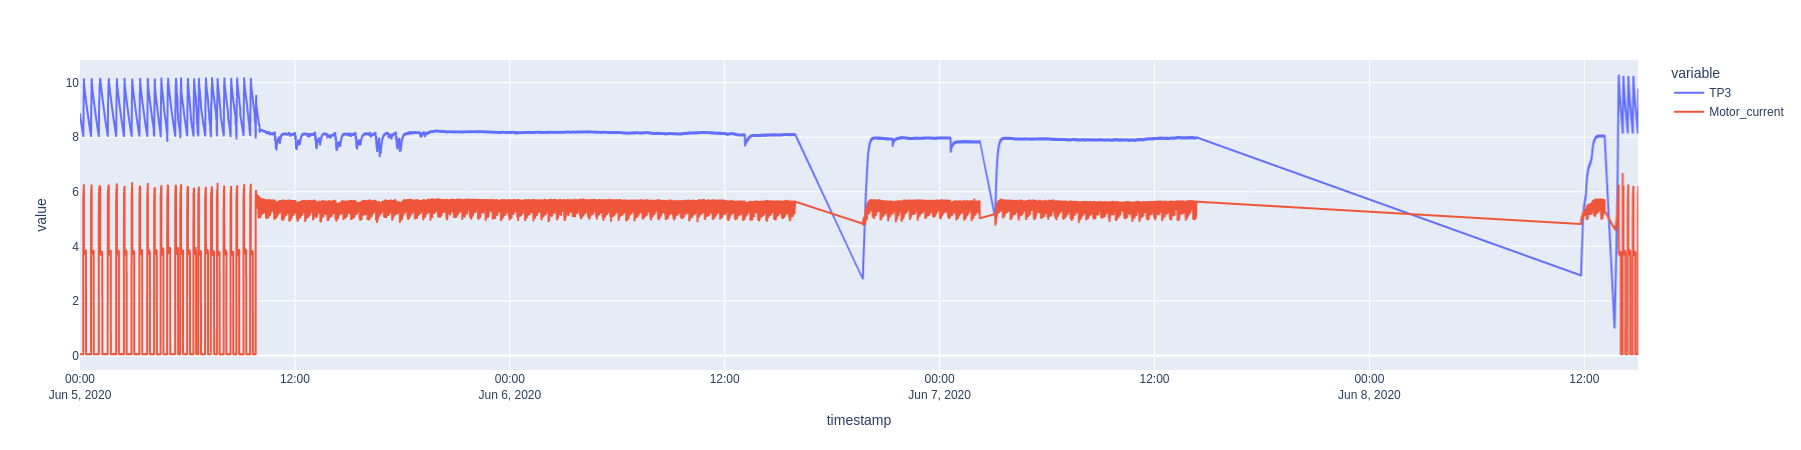
\includegraphics[width=\textwidth]{VisualizacionDatos.png}}
        \caption{Observamos los datos y los valores de la presión en el panel neumático (TP3, línea azul) y la corriente del motor (línea roja).}
        \label{fig:VisualizacionDatos}
\end{figure}

Se han recogido los resultados en la Tabla~\ref{tab:TiempoCiclo}. La mediana se calcula sobre los intervalos de tiempo no anómalos. No obstante, 
aunque el conjunto de datos no presenta valores pérdidos en ninguna de las columnas, sí que presenta saltos temporales. Los datos se mostrean cada 10 segundos, 
pero se ha encontrado saltos temporales de incluso días, véase Figura~\ref{fig:VentanaDeslizante}. Se planteó la posibilidad de interpolar los datos, pero dada la naturaleza 
del problema, serie temporal cíclica pero con intervalos distintos, es difícil obtener resultados prometedores sin la posibilidad de ``ensuciar'' la calidad de los datos.
Por ello, se ha calculado el tiempo mediano de ciclo de motor tras eliminar los saltos temporales. Para comprobar, se ha calculado también la mediana 
para todos intervalos sin anomalías de la Tabla~\ref{tab:Reportes}. Los valores obtenidos están en las cercanías del especificado en la Tabla~\ref{tab:TiempoCiclo}.

\begin{table}[!ht]
    \centering
    \begin{tabular}{|c|}
    \hline
    \textbf{Mediana del tiempo de ciclo} \\ \hline 
    1260 segundos\\
    \hline
    \end{tabular}
    \caption{Resultado obtenido del cálculo de la ventana deslizante. Se acerca a los obtenidos en el artículo original de detección de fallos de este dataset~\cite{FailureDetection}.}
    \label{tab:TiempoCiclo}
\end{table}

Para la asignación de los grupos se ha utilizado dos veces la mediana del tiempo de ciclo del motor. 
Esto es debido a que así se puede asegurar contener información de almenos más de la mitad de la activación del motor, asegurando que predecimos con la mayor información posible del estado del motor.
Se puede observar la asignación de grupos en la Figura~\ref{fig:VentanaDeslizante}.

\begin{figure}[!ht]
        \centering
        \subfloat{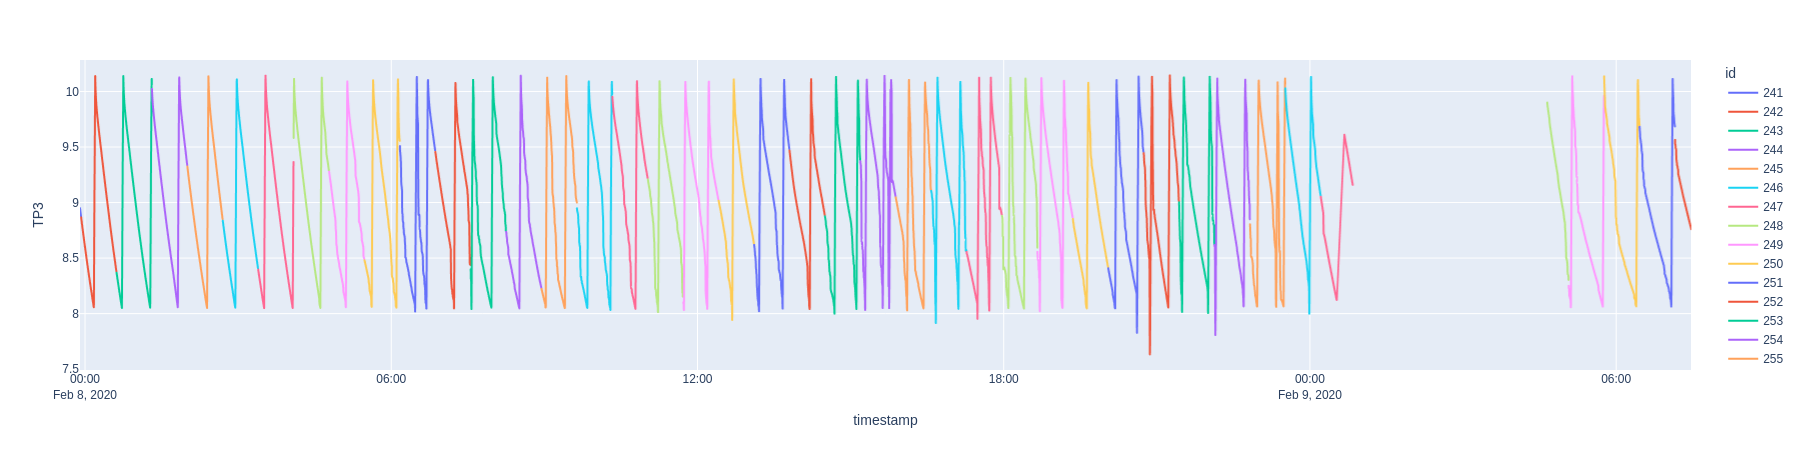
\includegraphics[width=\textwidth]{VentanaDeslizante.png}}
        \caption{Observamos los grupos asignados de utilizar 2 veces el tiempo de ciclo.}
        \label{fig:VentanaDeslizante}
\end{figure}


Durante el análisis EDA y prepración del conjunto de datos de entrenamiento y evaluación se han recogido nuevas anomalías, veáse la Tabla~\ref{tab:EventosRaros} y Figura~\ref{fig:EventosRaros}.
Sería interesante volver a consultar con un experto del campo para que valide dichas anomalías. No obstante, presentan un perfil suficientemente cercano al de las anomalías clasificadas.
Por ello, consideramos oportuno la inclusión de dichos ejemplos como anomalías para ayudar a paliar el bajo número de ejemplo de casos positivos.

\begin{table}[!ht]
    \centering
    \begin{tabular}{|c|l|l|r|l|}
    \hline
    \textbf{Número} & \textbf{Inicio}       & \textbf{Fin}         & \textbf{Duración (min)} & \textbf{Importancia} \\ \hline
    22 & 2020-03-06 21:42:15 & 2020-03-06 23:14:00 & 92 & - \\ \hline
    23 & 2020-03-11 05:15:10 & 2020-03-11 06:25:00 & 70 & - \\ \hline
    24 & 2020-03-12 00:15:56 & 2020-03-12 11:59:00 & 704 & - \\ \hline
    25 & 2020-03-26 04:00:20 & 2020-03-26 05:20:00 & 80 & - \\ \hline
    26 & 2020-03-27 07:12:00 & 2020-03-27 12:01:00 & 289 & - \\ \hline
    27 & 2020-04-17 08:50:28 & 2020-04-17 23:59:00 & 909 & - \\ \hline
    28 & 2020-04-25 00:07:15 & 2020-04-25 01:10:00 & 63 & - \\ \hline
    29 & 2020-05-19 01:35:28 & 2020-05-19 02:40:00 & 64 & - \\ \hline
    30 & 2020-06-12 01:41:07 & 2020-06-12 17:06:00 & 925 & - \\ \hline
    31 & 2020-07-21 13:32:48 & 2020-07-21 22:03:00 & 510 & - \\ \hline
    32 & 2020-07-22 06:40:46 & 2020-07-22 13:10:00 & 389 & - \\ \hline
    33 & 2020-07-31 00:57:33 & 2020-07-31 02:09:00 & 71 & - \\ \hline
    \end{tabular}
    \caption{Intervalos de tiempo encontrados con valores constantes y fluctuaciones extrañas, un patrón similar al de las anomalías, sin etiquetado.}
    \label{tab:EventosRaros}
\end{table}

\begin{figure}[!ht]
        \centering
        \subfloat{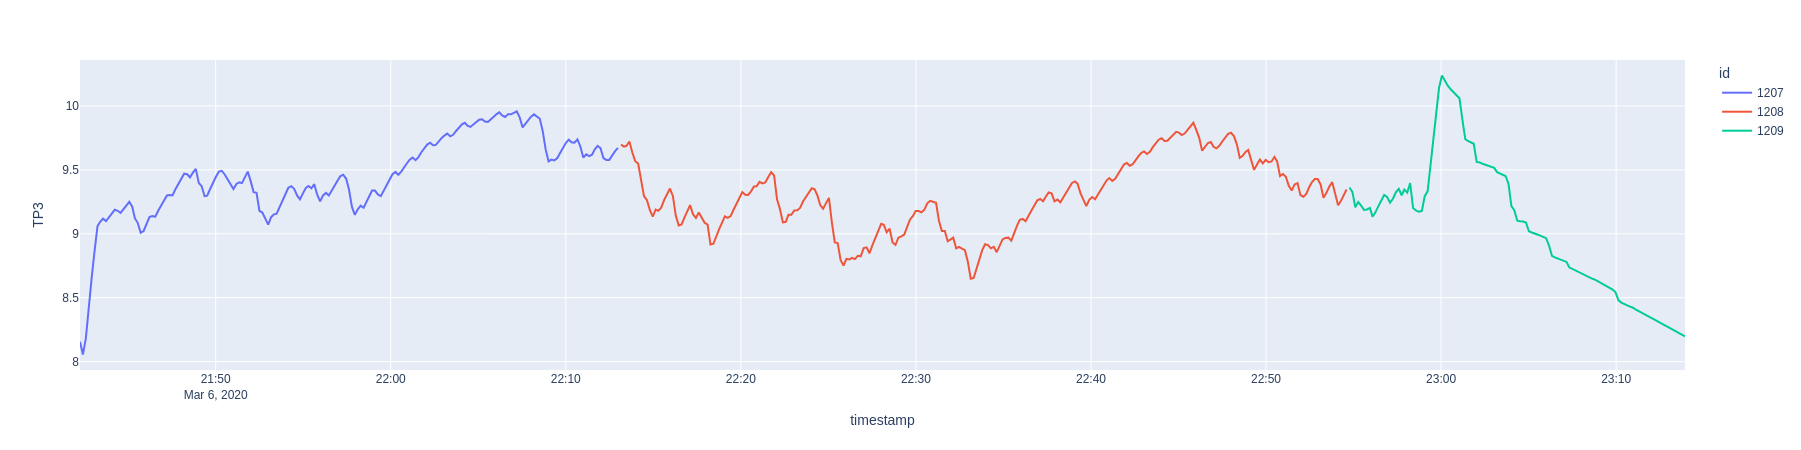
\includegraphics[width=\textwidth]{EjemploRaro1.png}}\\
        \subfloat{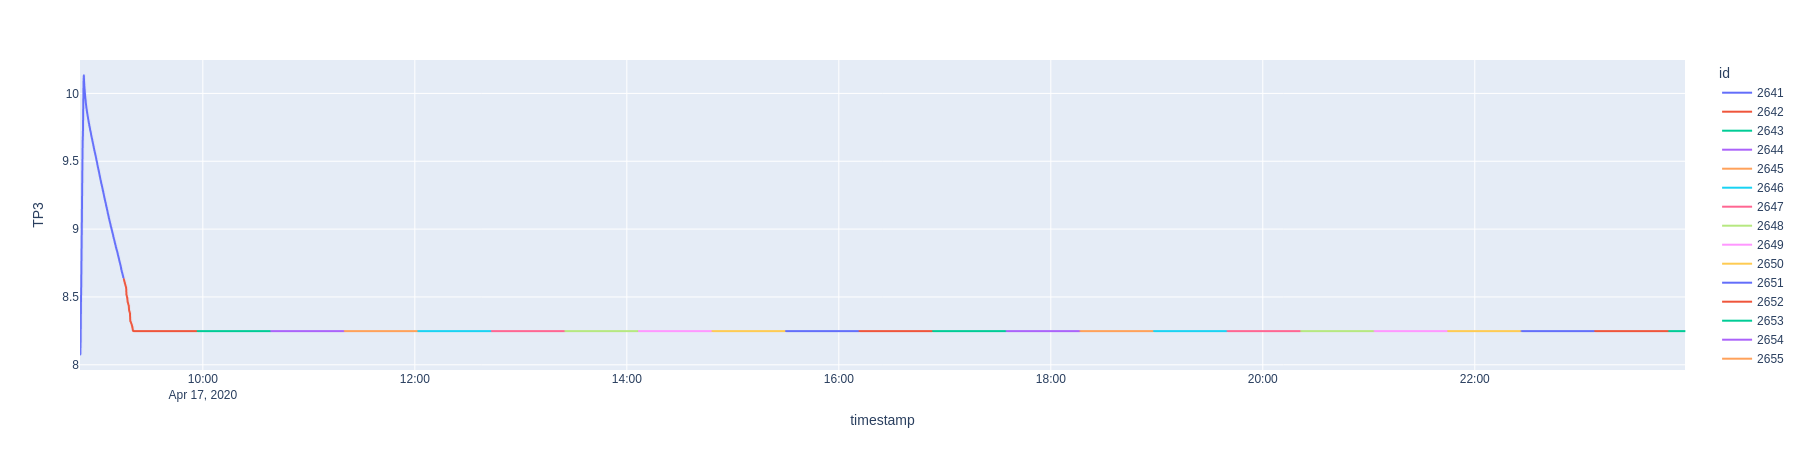
\includegraphics[width=\textwidth]{EjemploRaro2.png}}
        \caption{Ejemplo de nuevos intervalos anómalos encontrados. Observamos valores constantes o fluctuaciones fuera de lo habitual para el motor apagado o encendido.}
        \label{fig:EventosRaros}
\end{figure}

Tras observar y analizar el conjunto de datos, seguimos un acercamiento similar a~\cite{PredictiveMaintenance,FailureDetection} para tratar a la serie temporal, 
se ha optado por la transformación de los intervalos de las ventanas deslizante en obtener el promedio, mínimo, máximo y varianza de cada variable durante el intervalo de tiempo mostreado. 
Para resolver el problema de saltos temporales se ha eliminado aquellos conjuntos en los que se estiman estas variables para un número de puntos inferior a $(\textrm{tiempo de ciclo}) / 10 = 126$. Ya que esos ejemplos 
son estimados con menos puntos que el tiempo de activación del motor, lo cuál puede generar estimaciones del promedio y varianza sub-óptimos.

Una vez determinado la ventana deslizante y las características a extraer, se generar el conjunto de entrenamiento y evaluación. 
Para determinar si un intervalo de la ventana deslizante es una anomalía o no se ha utilizado un criterio de votación en el cuál gana la mayoría.
Para generar los conjuntos de datos, primeramente barajamos las ventanas deslizantes para asignar de forma aleatoria diferentes intervalos de tiempo en cada partición, 
evitando así pliegues más fáciles o difíciles (obtener unos resultados más balanceados en general). A continuación, se decide dividir los datos en 9 pliegues. 
se estima el número de anomalías que pertenecería a cada pliegue y se genera conjuntos lo más equilibrado posible (véase la Tabla~\ref{tab:Dataset}. 
Por último, se asigna el pliegue 1 y 8 (elección aleatoria) como el conjunto de test. Los resultantes serán agrupado en 4 pliegues para el entrenamiento de la validación cruzada. 

\begin{table}[!ht]
    \centering
    \begin{tabular}{|c|c|c|c|}
    \hline
    \textbf{Pliegue} & \textbf{Negativo} & \textbf{Positivo} & \textbf{Conjunto}\\ \hline
    0 & 635 & 31 & Evaluación \\ \hline
    1 & 635 & 31 & Etrenamiento pliegue 1 \\ \hline
    2 & 635 & 31 & Etrenamiento pliegue 2\\ \hline
        3 & 635 & 31 & Etrenamiento pliegue 3\\ \hline
        4 & 635 & 31 & Etrenamiento pliegue 4\\ \hline
        5 & 635 & 31 & Etrenamiento pliegue 3\\ \hline
        6 & 635 & 31 & Etrenamiento pliegue 2 \\ \hline
        7 & 638 & 31 & Etrenamiento pliegue 1\\ \hline
        8 & 641 & 43 & Evaluación \\ \hline
    \end{tabular}
    \caption{Distribución de los 9 pliegues generados. Se asigna de forma aleatoria el 1 y 8 a test. Se agrupan los demás hasta forma 4 pliegues usando el primer y último de los restantes: 0 y 7, 2 y 6, 5 y 3, 4.}
    \label{tab:ValidacionCruzada}
\end{table}

\section{Regresión Logística.}
\section{Máquinas de Vectores de Soporte.}
\section{Clasificador Bayesiano.}
\section{Árboles de clasificación.}
\section{Gradient Boosting.}
\section{Stacking.}
\section{AdaBoost.}
\section{Bagging.}
\printbibliography
\end{document}
